\documentclass[11pt,a4paper]{article}

% ---------------------------------------------------------------------------
% Complete enumeration of irreducible autocatalytic sets with bounded
% supplier choice.
%
% Author metadata: set the macros below before submission.  They are left
% blank deliberately.  \CompanionAuthor fills the author field of the
% companion-manuscript and repository citations in refs.bib.
% ---------------------------------------------------------------------------
\newcommand{\PaperAuthor}{}
\newcommand{\PaperAffiliation}{}
\newcommand{\PaperDate}{14 September 2026}
\newcommand{\CompanionAuthor}{Anonymous}

\usepackage[T1]{fontenc}
\usepackage[utf8]{inputenc}
\usepackage{lmodern}
\usepackage{microtype}
\usepackage[a4paper,margin=1.05in]{geometry}
\usepackage{amsmath,amssymb,amsthm,mathtools}
\usepackage{booktabs}
\usepackage{array}
\usepackage{enumitem}
\usepackage{xcolor}
\usepackage{graphicx}
\usepackage{tikz}
\usetikzlibrary{arrows.meta,positioning,calc}
\renewcommand{\topfraction}{0.9}
\renewcommand{\textfraction}{0.05}
\renewcommand{\floatpagefraction}{0.75}
\usepackage[obeyspaces,spaces]{url}
\usepackage[numbers,sort&compress]{natbib}
\usepackage[colorlinks=true,linkcolor=blue!55!black,citecolor=blue!55!black,urlcolor=blue!55!black]{hyperref}
\hypersetup{pdftitle={Complete enumeration of irreducible autocatalytic sets with bounded supplier choice},
 pdfauthor={\PaperAuthor},
 pdfsubject={Fixed-parameter enumeration of irreducible RAFs in catalytic reaction systems},
 pdfkeywords={autocatalytic sets, RAF theory, irreducible RAFs, enumeration, fixed-parameter tractability, hitting sets, formal verification}}

\providecommand{\doi}[1]{}
\renewcommand{\doi}[1]{\href{https://doi.org/#1}{\nolinkurl{doi:#1}}}

\setlist{itemsep=2pt,topsep=3pt}
\setlength{\emergencystretch}{1.5em}

\theoremstyle{plain}
\newtheorem{theorem}{Theorem}[section]
\newtheorem{proposition}[theorem]{Proposition}
\newtheorem{lemma}[theorem]{Lemma}
\newtheorem{corollary}[theorem]{Corollary}
\theoremstyle{definition}
\newtheorem{definition}[theorem]{Definition}
\newtheorem{example}[theorem]{Example}
\theoremstyle{remark}
\newtheorem{remark}[theorem]{Remark}
\newtheorem{question}[theorem]{Question}

\DeclareUrlCommand\lean{\urlstyle{tt}}

\newcommand{\Irr}{\mathcal I}
\newcommand{\cl}{\operatorname{cl}}
\newcommand{\muQ}{\mu_Q}
\newcommand{\Cat}{\operatorname{Cat}}
\newcommand{\inp}{\operatorname{in}}
\newcommand{\out}{\operatorname{out}}
\newcommand{\OPT}{\operatorname{OPT}}
\newcommand{\Nat}{\mathbb N}
\newcommand{\bmax}{\beta_{\max}}
\newcommand{\Closed}{\operatorname{Closed}}

\title{Complete enumeration of irreducible autocatalytic sets\\ with bounded supplier choice}
\author{\PaperAuthor\\ \PaperAffiliation}
\date{\PaperDate}

\begin{document}
\maketitle

\begin{abstract}
An irreducible reflexively autocatalytic and food-generated set (irreducible RAF, or irrRAF) is an inclusion-minimal nonempty RAF of a finite catalytic reaction system. A companion classification shows that no uniform output-polynomial algorithm lists the complete family of irrRAFs unless $\mathrm P=\mathrm{NP}$, so unconditional tractability must come from structure in the input. We identify such structure in the multiplicity of \emph{suppliers}. After polynomial maximal-RAF pruning, let $d_x$ be the number of reactions producing a nonfood species $x$ and let $a_r$ be the number of effective catalyst alternatives of a reaction $r$ (one, when a food catalyst is available). The supplier excess $\beta=\sum_x(d_x-1)+\sum_r(a_r-1)$ is computed from the input and bounds the number $L=\prod_xd_x\prod_ra_r\le2^\beta$ of deterministic supplier resolutions. We prove that every irrRAF survives at least one resolution, chosen by a globally shared earliest-producer rule; that the irrRAFs of a pruned resolution are exactly the sink strongly connected components of its consumer-to-supplier dependency graph; and that validating each such component in the original system, with one maximal-RAF call per reaction, yields precisely the complete original family. The algorithm runs in time and space $2^\beta N^{O(1)}$ for explicit input length $N$; it places no bound on the length of food-generation chains, so arbitrarily large deterministic systems have $\beta=0$. Because the components of one resolution are disjoint, every reaction lies in at most $L$ irrRAFs and the total output length is at most $mL$ for a maximal RAF of $m$ reactions; a coupled gate family shows that both bounds are attained up to a constant factor. Deleting reactions filters the family exactly and cannot increase $\beta$; incidence-separated components let the parameter be replaced by its largest local value, giving fixed-parameter tractability in $\bmax$; and destructive reaction sets are exactly the transversals of the catalogue, which yields a $(1+\beta\ln 2)$-approximate greedy intervention and exact cut-cost, cut-count and reliability formulas at zero excess. The catalogue theorem, its candidate bounds, the overlap bounds and the restriction identity are machine-checked in Lean~4; the cost, component and intervention results have conventional proofs. Bounded exact tests and an instrumented implementation illustrate the mechanisms.
\end{abstract}

\noindent\textbf{Keywords.} autocatalytic sets; RAF theory; irreducible RAFs; enumeration algorithms; fixed-parameter tractability; hitting sets; set cover; formal verification.

\medskip
\noindent\textbf{MSC 2020.} 92E20, 68Q27, 05C85, 68W40, 68V20.

\section{Introduction}\label{sec:intro}

Reflexively autocatalytic and food-generated sets (RAFs) are a finite combinatorial model of collectively self-sustaining reaction networks. The concept originates in Kauffman's autocatalytic sets of proteins \cite{kauffman1986autocatalytic}, was given its present form by Hordijk and Steel \cite{hordijk2004detecting}, and has grown into a structural theory with efficient algorithms and applications to early metabolism and the origin of life \cite{hordijk2012structure,hordijk2015algorithms,steel2019autocatalytic,sousa2015ecoli,xavier2020autocatalytic}. A catalytic reaction system consists of molecule types, reactions with reactants and products, a food set of freely available molecules, and a catalysis relation. A nonempty reaction set is a RAF if all of its reactants can be built up from the food by reactions of the set and each of its reactions is catalysed by a food molecule or by a molecule the set produces.

Unions of RAFs are RAFs, so a system containing a RAF contains a largest one, the \emph{maximal RAF}, computable in polynomial time by the RAF algorithm of Hordijk and Steel \cite{hordijk2004detecting}. The minimal organizations point the other way. Steel, Hordijk and Smith \cite{steel2013minimal} studied \emph{irreducible} RAFs (irrRAFs), which contain no proper RAF, and showed that one irrRAF can be found in polynomial time by a deletion sweep while a RAF of minimum size is NP-hard to find. They also gave a criterion certifying that a supplied list of $k$ irrRAFs is complete, at a cost growing as the product of the listed sizes, and asked whether this dependence can be improved \cite[Section~6.1]{steel2013minimal}. Hordijk's recent preprint develops exhaustive and randomized enumeration procedures \cite{hordijk2026enumerating}. A companion manuscript settles the unrestricted question: a uniform deterministic algorithm that writes every irrRAF exactly once in time polynomial in the input and output lengths exists if and only if $\mathrm P=\mathrm{NP}$ \cite{classification2026}; exact certification of a supplied family is coNP-complete, and its parameterized version is co-W[P]-complete \cite{certification2026}. Under standard assumptions the complete family is therefore out of reach for arbitrary inputs, and the practical question becomes which computable features of a reaction system make it reachable.

This paper answers that question for one natural feature: the multiplicity of \emph{suppliers}. In a system where every nonfood species has exactly one producer and every reaction has exactly one relevant catalyst, the requirements of a reaction determine the reactions it depends on, and inclusion-minimal RAFs become a graph problem. When some species have several producers or some reactions several catalysts, each alternative is a binary choice that the complete family may or may not exploit. We measure this ambiguity by the \emph{supplier excess} $\beta$ (Definition~\ref{def:beta}) and show that the complete irrRAF family can be listed exactly in time $2^\beta N^{O(1)}$. The parameter is measured on the input after one polynomial pruning, never on the unknown output, and it places no restriction on how long a chain of food-generation steps may be: a linear chain of a thousand reactions, each producing the reactant of the next, has $\beta=0$.

\subsection{Main results}

Throughout, $Q$ is a finite catalytic reaction system with reaction identifier set $R$, $\Irr(Q)$ is its family of irrRAFs, $K$ is its maximal RAF, $m=|K|$, $n=|R|$, and $N$ is the length of an explicit encoding of $Q$ (Section~\ref{sec:defs}). The supplier excess $\beta$ and the resolution count $L\le2^\beta$ are defined in Section~\ref{sec:parameter}.

\begin{itemize}
\item \textbf{Complete enumeration (Theorem~\ref{thm:main}, Proposition~\ref{prop:cost}).} A supplier catalogue algorithm returns exactly $\Irr(Q)$, each member once, in total time and space $2^\beta N^{O(1)}$. It inspects at most $mL$ candidate sets in total, and validates candidates with at most $m$ original maximal-RAF calls per resolution.
\item \textbf{Overlap bounds (Theorem~\ref{thm:main}).} $\Irr(Q)$ can be partitioned into at most $L$ classes of pairwise disjoint sets. Hence every reaction lies in at most $L$ irrRAFs, and $|\Irr(Q)|\le\sum_{I\in\Irr(Q)}|I|\le mL\le m2^\beta$.
\item \textbf{Sharpness (Proposition~\ref{prop:sharp}).} A family of systems with $3k$ reactions and $\beta=k$ has exactly $2^k$ irrRAFs, each of size $2k$, and each of its $k$ gate reactions lies in all of them. Any algorithm that writes every irrRAF explicitly needs time exponential in $\beta$ on this family.
\item \textbf{Restriction (Theorem~\ref{thm:restrict}).} Deleting reactions filters the family exactly, $\Irr(Q|U)=\{I\in\Irr(Q):I\subseteq U\}$, and cannot increase $\beta$. Counting, minimum-size and minimum-nonnegative-cost RAFs, required/forbidden queries and deletion survival are then direct scans of the catalogue.
\item \textbf{Components (Theorem~\ref{thm:components}).} If the nonfood incidence graph of the pruned system splits into blocks, the family is the disjoint union of the block families, $\beta$ adds and $L$ multiplies, but the algorithm pays the \emph{sum} of the block resolution counts. Enumeration is fixed-parameter tractable in the largest local excess $\bmax$.
\item \textbf{Interventions (Corollary~\ref{cor:greedy}, Theorem~\ref{thm:zero}).} A reaction set destroys every RAF exactly when it meets every irrRAF. Weighted greedy deletion is within a factor $H_d\le1+\ln L\le1+\beta\ln2$ of the cheapest destructive set. At $\beta=0$ the irrRAFs are pairwise disjoint and the optimal cut cost, the number of inclusion-minimal cuts and the probability that a RAF survives independent reaction failures have closed forms.
\end{itemize}

The enumeration theorem, its candidate and resolution bounds, both overlap bounds and the restriction identity are checked in Lean~4 \cite{demoura2021lean4,mathlib2020} with no hypotheses beyond the standard axioms (Section~\ref{sec:formal}). The complexity account, the monotonicity of $\beta$ under restriction, the component theorem and the intervention results are conventional proofs from those verified statements and are labelled as such.

\subsection{Proof idea}

A \emph{resolution} chooses one producer for each nonfood species and one effective catalyst for each reaction, deletes every other product occurrence, and replaces every catalyst list by its chosen member. Three facts make resolutions useful.

\emph{Soundness.} Thinning products and catalysts can only shrink food closures, so every RAF of a resolved system is a RAF of the original.

\emph{Preservation by earliest producers.} Fix an original RAF $I$. For each nonfood molecule in the closure of $I$, choose a producer in $I$ whose reactants are all present at the stage \emph{before} the molecule first appears, and use that one producer at every later stage. This single global choice per molecule keeps every closure stage of $I$ exactly equal to the original one, so $I$ remains a RAF, and by soundness an irreducible $I$ remains irreducible. An arbitrary producer choice does not suffice: choosing the self-loop $x\to x$ as the only producer of $x$ destroys the ability to start from food (Example~\ref{ex:earliest}).

\emph{Sink components.} In a resolution pruned to its maximal RAF, every required nonfood molecule has a unique producer. Drawing an arc from each reaction to the producer of each of its nonfood reactants and of its chosen catalyst, the RAFs are exactly the nonempty sets closed under outgoing arcs, and the irrRAFs are exactly the sink strongly connected components. Such components are disjoint and there are at most $m$ of them.

Every original irrRAF therefore appears as a sink component of some resolution. The converse fails: a sink component may be an original RAF that is no longer minimal once the deleted alternatives are restored (Figure~\ref{fig:filter}). A single original maximal-RAF call per reaction of the candidate decides this, and the disjointness of components charges those calls to disjoint reactions. The same disjointness gives the overlap bounds and, through a hitting-set reduction, the intervention guarantees.

\subsection{Related work}

\emph{Structural tractability in RAF theory.} Steel and Hordijk \cite{steel2018tractable} study elementary systems, in which every reactant is food, and characterize their irrRAFs through chordless cycles in a catalysis graph. Elementary systems remove nonfood generation; supplier bounds keep generation chains of any length and instead control alternative witnesses. Neither ``one catalyst per reaction'' nor ``one producer per molecule'' alone gives the present theorem: the companion SAT source of \cite{classification2026} has one catalyst per reaction and carries all of its choices through alternative producers, while its set-cover source carries choices through catalysis, so both excess terms are needed.

\emph{Enumeration complexity.} The output-sensitive standard for listing problems goes back to Johnson, Yannakakis and Papadimitriou \cite{johnson1988generating}; see Strozecki \cite{strozecki2023enumeration} for a survey of incremental time, delay and space. The present algorithm is a total-time bound with a parameter-dependent exponential factor, not an output-polynomial or polynomial-delay guarantee, and Section~\ref{sec:cost} says precisely what is and is not claimed about delay.

\emph{Parameterized complexity.} Fixed-parameter tractability with respect to a parameter measured on the input is the framework of Downey and Fellows \cite{downey2013fundamentals} and Cygan et al.\ \cite{cygan2015parameterized}. Courcelle's theorem \cite{courcelle1990monadic} and its enumeration form \cite{courcelle2009linear} give a general logical baseline for bounded-width inputs; Section~\ref{sec:width} records a monadic second-order translation of original irreducibility and shows that supplier excess and incidence treewidth are incomparable parameters.

\emph{Hitting sets and set cover.} Destructive reaction sets are transversals of the catalogue hypergraph. The greedy set-cover guarantee is due to Johnson, Lov\'asz and Chv\'atal \cite{johnson1974approximation,lovasz1975ratio,chvatal1979greedy} and is essentially optimal in general \cite{feige1998threshold,dinur2014analytical}; our contribution is the exact reduction and the structural bound on set sizes. Listing all minimal destructive cuts is the transversal hypergraph problem \cite{eiter1995identifying}, for which Fredman and Khachiyan give an incremental quasi-polynomial algorithm \cite{fredman1996complexity}.

\subsection{Evidence levels and organization}

Three kinds of evidence appear and are kept apart. Universal finite statements checked in Lean are named with their declarations in Section~\ref{sec:formal}. Conventional proofs are complete mathematical arguments in this paper that have not been ported to Lean. Computations are bounded exact tests and instrumented runs of a Python implementation that is not extracted from Lean; they illustrate and discriminate, but do not prove.

Section~\ref{sec:defs} fixes the model, maximal-RAF pruning, effective catalysts and the parameter. Section~\ref{sec:resolutions} develops resolutions, earliest producers, dependency graphs and sink components. Section~\ref{sec:enumeration} states the algorithm, the enumeration and overlap theorem and the cost bound. Section~\ref{sec:sharp} gives the sharpness family and zero-excess families of unbounded size, depth and width. Sections~\ref{sec:restriction}--\ref{sec:cuts} treat restriction and catalogue queries, independent components and interventions. Section~\ref{sec:formal} describes the formal development, Section~\ref{sec:experiments} the computational checks, and Section~\ref{sec:discussion} the scope of the result and open problems.

\section{Catalytic reaction systems and irreducible RAFs}\label{sec:defs}

\subsection{Closure and the RAF condition}

A \emph{catalytic reaction system} $Q=(M,R,F,\inp,\out,\Cat)$ consists of a finite set $M$ of molecule types, a finite set $R$ of reaction identifiers, a food set $F\subseteq M$, and for each $r\in R$ finite sets $\inp(r),\out(r),\Cat(r)\subseteq M$ of reactants, products and catalysts. Distinct identifiers remain distinct even if their incidence sets agree, and empty product sets are permitted; both conventions are used by the intermediate constructions below.

For $S\subseteq R$ the \emph{food closure} is computed in synchronous stages,
\begin{equation}\label{eq:closure}
 X_0(S)=F,\qquad
 X_{t+1}(S)=X_t(S)\cup\bigcup_{\substack{r\in S\\ \inp(r)\subseteq X_t(S)}}\out(r),
 \qquad \cl_Q(S)=\bigcup_{t\ge0}X_t(S).
\end{equation}
The stages stabilize because $M$ is finite. Catalysts do not gate this iteration. A nonempty $S\subseteq R$ is a \emph{RAF} if for every $r\in S$
\begin{equation}\label{eq:raf}
 \inp(r)\subseteq\cl_Q(S)\qquad\text{and}\qquad\Cat(r)\cap\cl_Q(S)\neq\varnothing.
\end{equation}
An \emph{irreducible RAF} (irrRAF) is a RAF with no proper RAF subset; $\Irr(Q)$ denotes the family of irrRAFs. If $S\subseteq T$ then $X_t(S)\subseteq X_t(T)$ for every $t$, by induction in \eqref{eq:closure}, so closures are monotone.

\begin{remark}[Semantic conventions]\label{rem:semantics}
Four conventions are essential and are those of the Lean development. (i)~Catalysts do not gate the closure: with food $f$, the single reaction $f\to x$ catalysed by $x$ is a RAF, although its first firing has no catalyst present; requiring catalytic startup is a stronger predicate. (ii)~Catalysis is disjunctive: one available member of $\Cat(r)$ suffices. (iii)~Irreducible means inclusion-minimal, not minimum cardinality; irrRAFs of one system may have different sizes. (iv)~Reactants and products record occurrence only. Stoichiometry, concentrations, rates, reversibility and conservation laws are outside the predicate. A set closed under the dependency arcs of Section~\ref{sec:resolutions} is not automatically a ``closed RAF'' in the separate RAF-theoretic sense of containing every reaction it enables.
\end{remark}

\subsection{Maximal RAFs and effective catalysts}\label{sec:maxraf}

For a container $U\subseteq R$ define $\muQ(U)$ by repeatedly removing from the current set every reaction that violates \eqref{eq:raf} with respect to the closure of the current set. At most $|U|$ strict removals occur. Every RAF $I\subseteq U$ survives every round, since its own closure is contained in the current closure; the fixed point is empty or a RAF, and it contains every RAF inside $U$. Thus $\muQ(U)$ is the unique maximal RAF in $U$ when one exists, and $\muQ$ is monotone in $U$. This is the RAF algorithm of \cite{hordijk2004detecting} restricted to a container.

Set $K=\muQ(R)$, $m=|K|$, $n=|R|$ and $M_K=F\cup\bigcup_{r\in K}\out(r)$. Every RAF is contained in $K$, and $\cl_Q(K)=M_K$: the inclusion $\subseteq$ is the closure definition, and every reaction of the RAF $K$ eventually fires, so all of its products appear. If $K=\varnothing$ both sides equal $F$.

For $x\in M_K\setminus F$ let $P_x=\{r\in K:x\in\out(r)\}$ be its producers in $K$ and $d_x=|P_x|\ge1$. For $r\in K$ fix
\begin{equation}\label{eq:effective}
 A_r=\begin{cases}
 \{\text{a fixed canonical member of }\Cat(r)\cap F\},&\Cat(r)\cap F\neq\varnothing,\\
 \Cat(r)\cap M_K,&\Cat(r)\cap F=\varnothing,
 \end{cases}\qquad a_r=|A_r|.
\end{equation}
The list $A_r$ is nonempty: a reaction of the RAF $K$ has a catalyst in $\cl_Q(K)=M_K$. The canonical choice uses a fixed order on species and adds no chemical condition.

\begin{lemma}[Effective catalysts]\label{lem:effective}
For every $S\subseteq K$, $S$ is a RAF of $Q$ if and only if $S$ is a RAF of the system obtained by replacing $\Cat(r)$ with $A_r$ for all $r\in K$.
\end{lemma}
\begin{proof}
Closures do not depend on catalysts. Food is in every closure, so a reaction with a food catalyst satisfies the catalyst condition in both systems. If $r$ has no food catalyst, $\cl_Q(S)\subseteq\cl_Q(K)=M_K$, so any catalyst of $r$ in $\cl_Q(S)$ lies in $\Cat(r)\cap M_K=A_r$. Every member of $A_r$ is an original catalyst.
\end{proof}

The lemma applies to every selected set inside $K$, not only to $K$ itself; that uniformity is what allows candidates to be tested for original minimality later.

\subsection{The supplier parameter}\label{sec:parameter}

\begin{definition}[Supplier excess and resolution count]\label{def:beta}
\begin{equation}\label{eq:beta}
 \beta(Q)=\sum_{x\in M_K\setminus F}(d_x-1)+\sum_{r\in K}(a_r-1),\qquad
 L(Q)=\prod_{x\in M_K\setminus F}d_x\prod_{r\in K}a_r .
\end{equation}
Empty products are $1$, so $K=\varnothing$ gives $\beta=0$, $L=1$ and $\Irr(Q)=\varnothing$.
\end{definition}

For every positive integer $b$ one has $b\le2^{b-1}$, so multiplying over all coordinates gives
\begin{equation}\label{eq:Lbound}
 L\le2^{\beta}.
\end{equation}
The exact count $L$ is often much smaller than $2^\beta$: one species with $b$ producers contributes $b-1$ to $\beta$ but only a factor $b$ to $L$. Both quantities are computed from the input after one polynomial pruning; their bit lengths are polynomial in $N$.

\begin{example}[Deep systems with zero excess]\label{ex:chain}
Let $r_1\colon f\to x_1$ and $r_i\colon x_{i-1}\to x_i$ for $2\le i\le\ell$, all catalysed by $x_\ell$. Every nonfood species has one producer and every reaction one catalyst, so $\beta=0$. Any RAF must generate $x_\ell$, which forces the whole chain, so the unique irrRAF has $\ell$ reactions and its closure needs $\ell$ stages. Supplier excess bounds neither the size of an output nor the depth of its generation.
\end{example}

\begin{remark}[Encoding]\label{rem:encoding}
Let $N$ be the bit length of an indexed explicit encoding of $M$, $R$, $F$ and the three incidence lists. Let $T_\mu(N)$ be a polynomial bound on one maximal-RAF computation, enlarged to cover the construction of resolutions, graph scans and strongly connected components. Such a polynomial exists directly from the finite closure and pruning loops; strongly connected components take linear time in the graph size \cite{tarjan1972depth,sharir1981strong}.
\end{remark}

\section{Supplier resolutions}\label{sec:resolutions}

\subsection{Resolutions and soundness}

\begin{definition}[Resolution]\label{def:resolution}
A \emph{resolution} $\sigma=(p,c)$ chooses a producer $p(x)\in P_x$ for every $x\in M_K\setminus F$ and a catalyst $c(r)\in A_r$ for every $r\in K$. The \emph{resolved system} $Q_\sigma$ has reaction set $K$, the same food and reactant sets, product sets
\[
 \out_\sigma(r)=(\out(r)\cap F)\cup\{x\in\out(r)\setminus F:p(x)=r\},
\]
and catalyst sets $\Cat_\sigma(r)=\{c(r)\}$. There are exactly $L$ resolutions.
\end{definition}

A resolution is a combinatorial construction, not a chemical intervention: it selects which witness each requirement will use.

\begin{lemma}[Soundness]\label{lem:sound}
For every resolution $\sigma$ and every $S\subseteq K$, $X_t^{Q_\sigma}(S)\subseteq X_t^{Q}(S)$ for all $t$. Consequently every RAF of $Q_\sigma$ is a RAF of $Q$.
\end{lemma}
\begin{proof}
Induction on $t$ in \eqref{eq:closure}: resolved product sets are subsets of the original ones, and a reaction enabled at a resolved stage is enabled at the corresponding original stage by the induction hypothesis. Every resolved catalyst $c(r)$ is an original catalyst, so both conditions of \eqref{eq:raf} transfer.
\end{proof}

\subsection{Earliest producers preserve every RAF}

\begin{lemma}[Earliest producers]\label{lem:earliest}
Let $S\subseteq K$ and let $x\notin F$ lie in $\cl_Q(S)$. There is a reaction $p\in S$ with $x\in\out(p)$ such that for every $t$, if $x\in X_{t+1}(S)$ then $\inp(p)\subseteq X_t(S)$.
\end{lemma}
\begin{proof}
Let $u+1$ be the first stage containing $x$; $u+1\ge1$ since $x\notin F$. Some $p\in S$ with $\inp(p)\subseteq X_u(S)$ produces $x$ at that stage. If $x\in X_{t+1}(S)$ then $t\ge u$, and stages are monotone in $t$, so $\inp(p)\subseteq X_u(S)\subseteq X_t(S)$.
\end{proof}

The point is that the same $p$ serves at \emph{every} later stage and for every consumer of $x$; a collection of unrelated witnesses, one per requirement, would not give a single producer function.

\begin{lemma}[Preserving resolution]\label{lem:preserve}
For every original RAF $I$ there is a resolution $\sigma$ such that $X_t^{Q_\sigma}(I)=X_t^{Q}(I)$ for all $t$ and $I$ is a RAF of $Q_\sigma$. If $I$ is an original irrRAF, then $I$ is an irrRAF of $Q_\sigma$.
\end{lemma}
\begin{proof}
For each $x\in\cl_Q(I)\setminus F$ let $p(x)\in I$ be a producer as in Lemma~\ref{lem:earliest}; note $p(x)\in P_x$ because $I\subseteq K$. For every other $x\in M_K\setminus F$ choose any member of $P_x$. We claim $X_t^{Q_\sigma}(I)=X_t^{Q}(I)$ for every $t$ and every catalyst choice $c$. The inclusion $\subseteq$ is Lemma~\ref{lem:sound}. For $\supseteq$ induct on $t$; stage $0$ is $F$ on both sides. Let $x\in X_{t+1}(I)$. If $x\in F$ it is present. Otherwise Lemma~\ref{lem:earliest} gives $\inp(p(x))\subseteq X_t(I)=X_t^{Q_\sigma}(I)$, so $p(x)$ fires at resolved stage $t$, and it retains the product $x$ because $p(x)$ is the chosen producer. Hence $x\in X_{t+1}^{Q_\sigma}(I)$.

For $r\in I$ choose $c(r)$ as the canonical food catalyst if $\Cat(r)\cap F\ne\varnothing$, and otherwise any catalyst in $\Cat(r)\cap\cl_Q(I)$; this set is nonempty because $I$ is a RAF and is contained in $\Cat(r)\cap M_K=A_r$. For $r\in K\setminus I$ choose any member of $A_r$. Every reactant and every chosen catalyst of a reaction in $I$ lies in the preserved closure, so $I$ is a resolved RAF. If $I$ is originally irreducible and $J\subsetneq I$ were a resolved RAF, then $J$ would be an original RAF by Lemma~\ref{lem:sound}, a contradiction.
\end{proof}

No single resolution is claimed to preserve all RAFs at once. Lemma~\ref{lem:preserve} is an existence statement for each RAF separately, and the earliest-stage condition does real work.

\begin{example}[Arbitrary producer choice can remove food startup]\label{ex:earliest}
Let $F=\{f\}$, $r_0\colon f\to x$ and $r_1\colon x\to x$, both catalysed by $x$. Originally $\{r_0\}$ is a RAF. Choosing $r_1$ as the sole producer of $x$ deletes $x$ from the products of $r_0$; the closure of $\{r_0,r_1\}$ in the resolved system is $\{f\}$, and no resolved RAF exists. The earliest producer of $x$ in the closure of $\{r_0\}$ is $r_0$, and that choice preserves it.
\end{example}

\subsection{Deterministic dependency graphs and sink components}

Fix a resolution $\sigma$ and let $K_\sigma=\mu_{Q_\sigma}(K)$ be the maximal RAF of the resolved system. If a reaction $r\in K_\sigma$ has a nonfood reactant $x$, or a nonfood chosen catalyst $c(r)=x$, then $x\in\cl_{Q_\sigma}(K_\sigma)$ and, since thinning left one producer, $p(x)$ is the unique reaction of $K_\sigma$ producing $x$. The \emph{dependency graph} $G_\sigma$ has vertex set $K_\sigma$ and an arc $r\to p(x)$ for every nonfood reactant $x$ of $r$ and for its nonfood chosen catalyst. Arcs point from consumer to supplier; a reaction may have several outgoing arcs, and ``deterministic suppliers'' does not mean outdegree at most one. A set $S\subseteq K_\sigma$ is \emph{outgoing-closed} if every arc leaving a vertex of $S$ ends in $S$.

\begin{lemma}[Deterministic dependency characterization]\label{lem:det}
A nonempty $S\subseteq K_\sigma$ is a RAF of $Q_\sigma$ if and only if it is outgoing-closed in $G_\sigma$.
\end{lemma}
\begin{proof}
If $S$ is a RAF and $r\in S$ requires the nonfood molecule $x$ as reactant or chosen catalyst, then $x\in\cl_{Q_\sigma}(S)$, so some reaction of $S$ produces $x$; by uniqueness that reaction is $p(x)$, the head of the arc. Hence $S$ is outgoing-closed.

Conversely let $S$ be outgoing-closed and use the closure stages $X_t(K_\sigma)$ of the RAF $K_\sigma$. We show by strong induction on $t$: whenever $r\in S$ has $\inp(r)\subseteq X_t(K_\sigma)$, then $\inp(r)\subseteq\cl_{Q_\sigma}(S)$ and $\out_\sigma(r)\subseteq\cl_{Q_\sigma}(S)$. For $t=0$ the reactants are food. For the step, a nonfood reactant $x$ of $r$ first appeared at a stage $u+1\le t$ through its unique producer $p(x)$, whose reactants lie in $X_u(K_\sigma)$ with $u<t$. The arc $r\to p(x)$ keeps $p(x)\in S$, so by induction $x\in\cl_{Q_\sigma}(S)$. Thus $r$ fires in the closure of $S$ and its products appear. Since $K_\sigma$ is a RAF, every $r\in S$ has its reactants at some stage, so the reactant condition holds for all of $S$. The chosen catalyst of $r$ is food or the product of $p(c(r))\in S$, which fires by the same argument; so the catalyst condition holds. No catalyst was assumed to precede its consumer in generation time.
\end{proof}

Pruning to $K_\sigma$ is essential for the converse: a dependency cycle can be closed under outgoing arcs without any way to start from food, and the generation stages of $K_\sigma$ rule this out.

\begin{lemma}[Minimal sets are sink components]\label{lem:sink}
The irrRAFs of $Q_\sigma$ are exactly the sink strongly connected components of $G_\sigma$, isolated vertices included as singleton components. They are pairwise disjoint and there are at most $|K_\sigma|\le m$ of them.
\end{lemma}
\begin{proof}
In a finite digraph the set reachable from a vertex is nonempty and outgoing-closed. If $S$ is a minimal nonempty outgoing-closed set and $v\in S$, the set reachable from $v$ is contained in $S$ and is itself nonempty and outgoing-closed, hence equals $S$; so every vertex of $S$ reaches every other, and no arc leaves $S$: $S$ is a sink strongly connected component. Conversely a nonempty outgoing-closed subset of a sink component contains everything reachable from one of its vertices, that is, the entire component. Apply Lemma~\ref{lem:det}. Distinct strongly connected components are disjoint.
\end{proof}

\subsection{Original validation is necessary}\label{sec:validation}

\begin{figure}[tb]
\centering
\begin{tikzpicture}[>=Latex,font=\small,
  panel/.style={anchor=north west,align=left,text width=4.4cm,inner sep=0pt},
  head/.style={font=\small\bfseries,color=blue!45!black},
  rx/.style={draw=blue!45!black,rounded corners=2pt,inner sep=3pt,font=\small},
  arr/.style={->,thick,color=orange!80!black}]
\node[panel] (p1) at (0,0) {\textcolor{blue!45!black}{\textbf{Original system}}\\[4pt]
 $r_0\colon f\to x$, catalysts $\{x,y\}$\\
 $r_1\colon x\to y$, catalyst $\{x\}$\\[4pt]
 $\{r_0\}$ is already a RAF.};
\node[panel] (p2) at (5.4,0) {\textcolor{blue!45!black}{\textbf{Resolution choosing $y$ for $r_0$}}\\[4pt]
 \begin{tikzpicture}[baseline]
  \node[rx] (a) at (0,0) {$r_0$};
  \node[rx] (b) at (2.2,0) {$r_1$};
  \draw[->,thick] (a) to[bend left=25] node[above,font=\scriptsize]{catalyst $y$} (b);
  \draw[->,thick] (b) to[bend left=25] node[below,font=\scriptsize]{reactant $x$} (a);
 \end{tikzpicture}\\[2pt]
 Sink component $\{r_0,r_1\}$.};
\node[panel] (p3) at (10.8,0) {\textcolor{blue!45!black}{\textbf{Original validation}}\\[4pt]
 $\muQ(\{r_1\})=\varnothing$\\
 $\muQ(\{r_0\})=\{r_0\}\ne\varnothing$\\[4pt]
 Reject $\{r_0,r_1\}$; keep $\{r_0\}$.};
\draw[arr] (4.55,-0.9) -- (5.25,-0.9);
\draw[arr] (9.95,-0.9) -- (10.65,-0.9);
\end{tikzpicture}
\caption{Original validation is necessary. With food $f$, choosing the nonfood catalyst $y$ for $r_0$ creates a two-vertex dependency cycle whose sink component is a resolved irrRAF. Restoring the original alternative $x$ reveals the proper RAF $\{r_0\}$, so the pair is rejected by the one-deletion test \eqref{eq:validate}.}
\label{fig:filter}
\end{figure}

Lemmas~\ref{lem:preserve} and~\ref{lem:sink} show that every original irrRAF is a sink component of some resolution. The converse fails.

\begin{example}[Resolved minima need not be original minima]\label{ex:filter}
(a) Figure~\ref{fig:filter}: $r_0\colon f\to x$ with catalysts $\{x,y\}$ and $r_1\colon x\to y$ with catalyst $\{x\}$. Choosing $y$ for $r_0$ makes $\{r_0,r_1\}$ a sink component, but $\{r_0\}$ is an original RAF.
(b) Producer choices cause the same effect: $r_0\colon f\to\{x,z\}$ catalysed by $x$ and $r_1\colon f\to x$ catalysed by $z$. Choosing $r_1$ as the unique producer of $x$ deletes $x$ from $\out(r_0)$; the resolved system has the single irrRAF $\{r_0,r_1\}$, whereas $\{r_0\}$ is already an original RAF.
\end{example}

The original exact pilot of Section~\ref{sec:experiments} rejected $111$ such candidate occurrences among $2{,}065$; they are expected behaviour of a necessary filter, not exceptions to the theorem.

\section{The enumeration theorem}\label{sec:enumeration}

\subsection{Testing original irreducibility}

For a set $C$ already known to be an original RAF,
\begin{equation}\label{eq:validate}
 C\in\Irr(Q)\quad\Longleftrightarrow\quad \muQ(C\setminus\{r\})=\varnothing\ \text{ for every } r\in C .
\end{equation}
Indeed a proper RAF subset omits some $r$ and survives the pruning of $C\setminus\{r\}$; conversely a nonempty $\muQ(C\setminus\{r\})$ is a proper RAF subset. This is the one-deletion criterion of \cite{steel2013minimal}, applied inside the container $C$. It asks whether any RAF \emph{remains} after a deletion, not whether the immediate deletion is itself a RAF.

\begin{example}[Immediate deletion is the wrong test]\label{ex:immediate}
Let $a\colon f\to x$ have the food catalyst $f$, let $b\colon x\to y$ be catalysed by $z$, and let $c\colon x\to z$ be catalysed by $y$. The set $\{a,b,c\}$ is a RAF with closure $\{f,x,y,z\}$. None of $\{a,b\}$, $\{a,c\}$, $\{b,c\}$ is a RAF, yet $\{a\}$ is, so $\{a,b,c\}$ is reducible although every single deletion leaves a non-RAF. Criterion~\eqref{eq:validate} detects this because $\muQ(\{a,b\})=\{a\}\ne\varnothing$.
\end{example}

\subsection{The supplier catalogue algorithm}

\begin{center}
\fbox{\begin{minipage}{.93\linewidth}\small
\textbf{Supplier catalogue algorithm}\smallskip
\begin{enumerate}[leftmargin=1.6em]
\item Compute $K=\muQ(R)$ and the lists $P_x$ ($x\in M_K\setminus F$) and $A_r$ ($r\in K$). If $K=\varnothing$, return the empty catalogue.
\item For each resolution $\sigma\in\prod_xP_x\times\prod_rA_r$: construct $Q_\sigma$, compute $K_\sigma=\mu_{Q_\sigma}(K)$, build $G_\sigma$ and find its sink strongly connected components.
\item For each sink component $C$: test \eqref{eq:validate} in the \emph{original} system $Q$. Insert the original-identifier mask of every accepted $C$ into a binary trie \cite{fredkin1960trie}.
\item After all resolutions, return the distinct masks stored in the trie.
\end{enumerate}
\end{minipage}}
\end{center}

\subsection{Completeness and overlap}

For $r\in R$ let $f_r=|\{I\in\Irr(Q):r\in I\}|$ be the \emph{frequency} of $r$.

\begin{theorem}[Complete enumeration and overlap]\label{thm:main}
The supplier catalogue is exactly $\Irr(Q)$, each member returned once. At most $mL$ candidate occurrences are inspected in total. The family $\Irr(Q)$ can be partitioned into at most $L$ classes whose members are pairwise disjoint. Consequently
\begin{equation}\label{eq:incidence}
 f_r\le L\quad(r\in R),\qquad
 |\Irr(Q)|\le\sum_{I\in\Irr(Q)}|I|=\sum_{r\in K}f_r\le mL\le m2^{\beta}.
\end{equation}
\end{theorem}
\begin{proof}
Every accepted set is a RAF of some $Q_\sigma$, hence an original RAF by Lemma~\ref{lem:sound}, and passes \eqref{eq:validate}, hence lies in $\Irr(Q)$. Conversely, an original irrRAF $I$ is an irrRAF of a preserving resolution $\sigma$ by Lemma~\ref{lem:preserve}. It lies in $K_\sigma$ because $K_\sigma$ contains every RAF of $Q_\sigma$ inside $K$, it is a sink component by Lemma~\ref{lem:sink}, and it passes \eqref{eq:validate}. The trie removes duplicates without removing a distinct member.

Within one resolution the sink components are nonempty and pairwise disjoint, so there are at most $|K_\sigma|\le m$ of them; summing over the $L$ resolutions bounds the candidate occurrences. Fix an order of the resolutions and assign each $I\in\Irr(Q)$ to the first resolution in which it is a sink component. Sets assigned to one resolution are disjoint, which gives the partition. A reaction occurs in at most one set of each class, so $f_r\le L$; reactions outside $K$ have frequency $0$. Double counting the pairs $(r,I)$ with $r\in I$ gives the identity in \eqref{eq:incidence}, the first inequality uses that every irrRAF is nonempty, and the last is \eqref{eq:Lbound}.
\end{proof}

The assignment in the proof is a proper $L$-colouring of the intersection graph of the catalogue (vertices $\Irr(Q)$, edges between intersecting members). It is not a degree bound for that graph: one large member may meet many disjoint members of another class. If every output has at least $s\ge1$ reactions, \eqref{eq:incidence} gives $|\Irr(Q)|\le\lfloor mL/s\rfloor$. Frequencies count distinct minimal organizations; they are not probabilities of a reaction being active, and sampling resolutions uniformly does not sample irrRAFs uniformly, since different irrRAFs survive different numbers of resolutions.

\subsection{Cost}\label{sec:cost}

Within one resolution, criterion \eqref{eq:validate} makes at most
\[
 \sum_{C\text{ a sink component of }G_\sigma}|C|\ \le\ |K_\sigma|\ \le\ m
\]
original maximal-RAF calls, because the components are disjoint. This charges validation to disjoint reactions across the whole resolution instead of paying $m$ separately for each candidate.

\begin{proposition}[Conventional cost bound]\label{prop:cost}
With original $n$-bit masks, the supplier catalogue algorithm runs in time
\begin{equation}\label{eq:time}
 O\bigl(T_\mu(N)+L\,((m+1)\,T_\mu(N)+mn)\bigr)
\end{equation}
and uses $N^{O(1)}+O(mnL)$ bits of storage, up to polynomial identifier overhead. In particular both are $2^\beta N^{O(1)}$, with an exponent of the polynomial factor independent of $\beta$.
\end{proposition}
\begin{proof}
Preprocessing costs $O(T_\mu(N))$. Each resolution costs one resolved pruning, at most $m$ original validation prunings, and graph work absorbed into $T_\mu$. At most $m$ candidate occurrences are accepted per resolution, each requiring an $n$-step trie traversal; a trie creates at most one node per traversed bit. Only one resolved system need be kept at a time. Counters and indices have polynomial bit length since $\log_2L\le\beta\le N^{O(1)}$. Pessimistic implementations of finite-set operations add only an input-polynomial factor. Substitute \eqref{eq:Lbound}.
\end{proof}

\begin{remark}[What is and is not claimed about delay]\label{rem:delay}
The implementation buffers its catalogue: the time to the first output includes the entire construction, and later masks are emitted in $O(n)$ each. This gives parameter-dependent total time and parameter-dependent delay after preprocessing. It does not establish polynomial delay for unrestricted $\beta$, which by \cite{classification2026} would imply $\mathrm P=\mathrm{NP}$; nor polynomial space independent of $\beta$. Relabelling $K$ would replace $n$ by $m$ in \eqref{eq:time}, but the reported implementation keeps original identifiers, including those removed by the initial pruning. Sparse output lists have total length at most $mL$ by \eqref{eq:incidence}, although the simple trie uses more space.
\end{remark}

\begin{remark}[The parameter is sufficient, not necessary]\label{rem:sufficient}
Two reactions with distinct food reactants, the same $q$ nonfood products and a food catalyst have exactly two irrRAFs, the two singletons, but every shared product has two producers, so $\beta=q$ and $L=2^q$. Unused shared outputs create supplier coordinates that no RAF requirement exploits. Theorem~\ref{thm:main} remains correct and its bound is loose. A preprocessing step that deletes irrelevant products would need its own preservation proof and is not assumed by the algorithm.
\end{remark}

\section{Sharpness and zero-excess families}\label{sec:sharp}

\subsection{A family in which every supplier choice is essential}

For $k\ge1$ take food $f$, nonfood species $x_1,\ldots,x_k,z_1,\ldots,z_k$ and $3k$ reactions: two producers $a_i,b_i\colon f\to x_i$ for each $i$, and the gates
\[
 g_1\colon x_1\to z_1,\qquad g_i\colon z_{i-1}+x_i\to z_i\quad(2\le i\le k),
\]
where $+$ denotes a joint reactant requirement. Every reaction has the sole catalyst $z_k$.

\begin{proposition}[Exponential output and frequency]\label{prop:sharp}
This system has $m=3k$, $\beta=k$ and $L=2^k$. Its irrRAFs are exactly the $2^k$ sets consisting of all $k$ gates and one member of each pair $\{a_i,b_i\}$. Every gate has frequency $L$, every output has size $2k$, and $\sum_{I\in\Irr(Q)}|I|=2k2^k=\tfrac23mL$.
\end{proposition}
\begin{proof}
The whole system is a RAF, so $K=R$. Any RAF must generate its only catalyst $z_k$, whose unique producer is $g_k$; backwards along the gate chain, all gates and at least one producer of each $x_i$ are required. Conversely such a selection generates every $x_i$ at stage $1$, then $z_1,\ldots,z_k$ in order, so it is a RAF, and minimality removes every surplus pair member. Only the $k$ species $x_i$ have two producers; all catalysts and all gate products are unique. The counts follow.
\end{proof}

The two producers of $x_i$ may instead consume distinct food substrates $f_{i,0},f_{i,1}\in F$; the proof and all parameters are unchanged, so the phenomenon does not depend on chemically identical reactions. The family shows that an exponential dependence on $\beta$ is unavoidable for any algorithm required to write every irrRAF explicitly, that the frequency bound $f_r\le L$ of \eqref{eq:incidence} is attained, and that the total-membership bound $mL$ is attained within the factor $2/3$. It is not a lower bound for counting or for compressed representations. Figure~\ref{fig:gate} shows the case $k=2$, which is also the worked example of Section~\ref{sec:worked}.

\begin{figure}[tb]
\centering
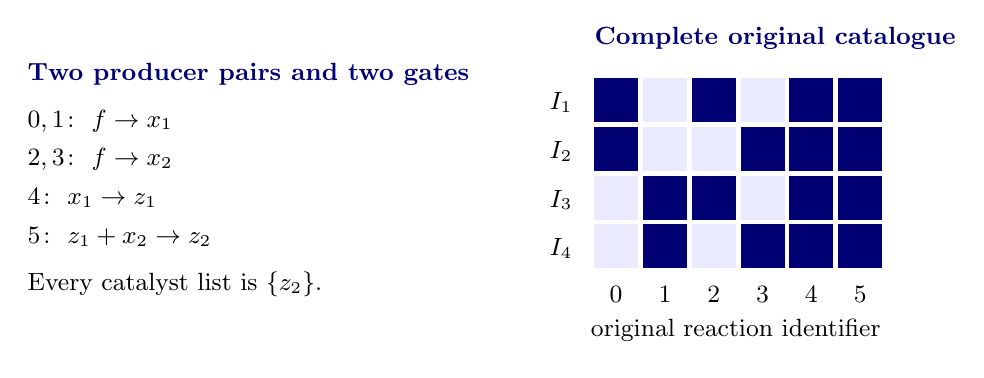
\begin{tikzpicture}[font=\small]
\node[anchor=north west,align=left,inner sep=0pt] at (0,2.6) {%
 \textcolor{blue!45!black}{\textbf{Two producer pairs and two gates}}\\[6pt]
 $0,1\colon\ f\to x_1$\\[3pt]
 $2,3\colon\ f\to x_2$\\[3pt]
 $4\colon\ x_1\to z_1$\\[3pt]
 $5\colon\ z_1+x_2\to z_2$\\[6pt]
 Every catalyst list is $\{z_2\}$.};
\begin{scope}[xshift=7.2cm,yshift=2.4cm]
 \node[anchor=south west,inner sep=0pt] at (0,0.35) {\textcolor{blue!45!black}{\textbf{Complete original catalogue}}};
 \foreach \row/\lab in {0/{$I_1$},1/{$I_2$},2/{$I_3$},3/{$I_4$}}{
   \node[anchor=east,font=\small] at (-0.15,-\row*0.62-0.31) {\lab};
 }
 \foreach \row/\a/\b/\c/\d/\e/\f in {0/1/0/1/0/1/1, 1/1/0/0/1/1/1, 2/0/1/1/0/1/1, 3/0/1/0/1/1/1}{
   \foreach \col/\v in {0/\a,1/\b,2/\c,3/\d,4/\e,5/\f}{
     \ifnum\v=1
       \fill[blue!45!black] (\col*0.62,-\row*0.62) rectangle ++(0.56,-0.56);
     \else
       \fill[blue!8] (\col*0.62,-\row*0.62) rectangle ++(0.56,-0.56);
     \fi
   }
 }
 \foreach \col in {0,...,5}{\node[font=\small] at (\col*0.62+0.28,-2.75) {\col};}
 \node[font=\small] at (1.8,-3.2) {original reaction identifier};
\end{scope}
\end{tikzpicture}
\caption{The $k=2$ gate construction with reaction identifiers $0,\ldots,5$. The four rows on the right are the complete original catalogue; dark cells are included reactions. Both gates occur in every output and each producer alternative occurs in two.}
\label{fig:gate}
\end{figure}

\subsection{Zero-excess families of unbounded size, depth and width}\label{sec:zerofamilies}

The following systems all have $\beta=0$ and therefore a single resolution, in which the irrRAFs are simply the sink components of one dependency graph.

\begin{example}[Attaining the factor $m$]
$m$ reactions $f\to x_i$, each catalysed by food, form $m$ disjoint singleton irrRAFs, so $|\Irr(Q)|=mL=m$ and \eqref{eq:incidence} is exact. This system also has $2^m-1$ RAFs in total: a small complete \emph{minimal} family does not imply a small family of all RAFs.
\end{example}

\begin{example}[Unbounded depth]
The chain of Example~\ref{ex:chain} has one irrRAF of size $\ell$ and generation depth $\ell$.
\end{example}

\begin{example}[Unbounded incidence treewidth]\label{ex:dense}
Replace the reactants of $r_i$ in Example~\ref{ex:chain} by $\{f,x_1,\ldots,x_{i-1}\}$, keeping the sole catalyst $x_\ell$. Producers and catalysts are still unique, so $\beta=0$, and the unique irrRAF is still the whole chain. But the reactions $r_{\lceil\ell/2\rceil+1},\ldots,r_\ell$ and the species $x_1,\ldots,x_{\lfloor\ell/2\rfloor}$ span a complete bipartite subgraph of the species--reaction incidence graph, whose treewidth therefore grows linearly in $\ell$.
\end{example}

Conversely, the gate family of Proposition~\ref{prop:sharp} has bounded width: the bags $B_i=\{f,z_k,x_i,z_i,g_i,a_i,b_i,z_{i-1}\}$ (with $z_0$ omitted) cover every reactant, product and catalyst incidence, consecutive bags share $z_i$, and $f,z_k$ lie in all bags, so the incidence graph has pathwidth at most $7$ while $\beta=k$ and the output is exponential. Supplier excess and incidence width are incomparable parameters (Section~\ref{sec:width}).

\section{Reaction restriction and catalogue queries}\label{sec:restriction}

For $U\subseteq R$ let $Q|U$ be the system with reaction set $U$, the same food, and the original incidence sets of the retained reactions. Retained identifiers are identified with their originals.

\begin{theorem}[Restriction and parameter monotonicity]\label{thm:restrict}
\begin{equation}\label{eq:restriction}
 \Irr(Q|U)=\{I\in\Irr(Q):I\subseteq U\},\qquad \beta(Q|U)\le\beta(Q).
\end{equation}
\end{theorem}
\begin{proof}
For $S\subseteq U$ the closure stages of $S$ in $Q|U$ and in $Q$ agree, so RAF membership agrees. If $I\subseteq U$ has a proper original RAF subset, that subset lies in $U$; conversely every proper restricted RAF subset is an original one. This is the family identity.

Write $K_U=\muQ(U)\subseteq K$, by monotonicity of $\muQ$. The nonfood species produced by $K_U$ are among those produced by $K$, and for each of them the producer list inside $K_U$ is a nonempty subset of the list inside $K$; so every surviving term $d_x-1$ does not increase and vanished species contribute $0$. For $r\in K_U$, whether $r$ has a food catalyst is unchanged, giving contribution $0$ in both systems; otherwise the effective list changes from $\Cat(r)\cap M_K$ to its subset $\Cat(r)\cap M_{K_U}$, nonempty because $r$ is supported in $K_U$. Removed reactions contribute $0$. Sum.
\end{proof}

Unchanged food and unchanged catalysis are hypotheses. Deleting a catalysis edge rather than a reaction can increase the excess: a single reaction $f\to\{x,y\}$ with catalysts $\{f,x,y\}$ has $\beta=0$, and removing only the food catalysis leaves a RAF with two effective nonfood catalysts and $\beta=1$. Equation~\eqref{eq:restriction} filters \emph{original} irrRAFs; it is not a search for sets minimal under an additional required-reaction constraint.

\subsection{Queries answered by the catalogue}

Once the catalogue is built, the following are direct scans, each polynomial in the catalogue size.
\begin{itemize}
\item \emph{Counting and minimum size.} $|\Irr(Q)|$ and $\min_I|I|$ are read off; every finite RAF contains an irrRAF, so the latter is the minimum RAF cardinality \cite{steel2013minimal}.
\item \emph{Minimum nonnegative cost.} For nonnegative additive reaction costs, a minimum-cost nonempty RAF may be taken irreducible, since replacing a RAF by an irreducible subset cannot increase cost. With signed costs this fails: for $a\colon f\to x$ and $b\colon x\to y$, both catalysed by $x$, the unique irrRAF is $\{a\}$ while the maximal RAF $\{a,b\}$ is cheaper when $c_b<0$. The same example shows $\bigcup\Irr(Q)\subsetneq K$ in general.
\item \emph{Required and forbidden reactions.} For disjoint $A,B\subseteq R$, the irrRAFs with $A\subseteq I$ and $I\cap B=\varnothing$ are the records passing the two filters.
\item \emph{Deletion survival.} By \eqref{eq:restriction} and finite minimal-subset existence, a RAF survives the deletion of $D\subseteq R$ if and only if some record is disjoint from $D$, and the surviving family is exactly the filtered catalogue. Survival alone is also answered by one maximal-RAF call; the catalogue adds the full list of alternatives.
\item \emph{Universally necessary reactions.} If $\Irr(Q)\ne\varnothing$, a reaction lies in every irrRAF exactly when deleting it destroys every RAF; this needs at most $n$ maximal-RAF calls and no enumeration \cite{classification2026}. For an empty family the vacuous intersection must be reported as ``no RAF'', not as necessity.
\end{itemize}

\subsection{A worked example}\label{sec:worked}

Take the $k=2$ system of Figure~\ref{fig:gate}: $F=\{f\}$, reactions $0,1\colon f\to x_1$, $2,3\colon f\to x_2$, $4\colon x_1\to z_1$, $5\colon z_1+x_2\to z_2$, all catalysed by $z_2$. Here $K=R$, $m=n=6$, $\beta=2$, $L=4$, and
\[
 \Irr(Q)=\bigl\{\{0,2,4,5\},\ \{0,3,4,5\},\ \{1,2,4,5\},\ \{1,3,4,5\}\bigr\},
\]
with frequencies $(2,2,2,2,4,4)$ summing to $16$. Both gates are universally necessary. Requiring $0$ and forbidding $2$ selects $\{0,3,4,5\}$ only; deleting $0$ leaves two alternatives. The inclusion-minimal destructive cuts are $\{4\}$, $\{5\}$, $\{0,1\}$ and $\{2,3\}$: a gate is hit, or both members of a producer pair are; a single alternative producer is never destructive.

With deletion costs $(c_0,\ldots,c_5)=(2,3,4,1,7,6)$ the four minimal cuts cost $7,6,5,5$, so the optimum is $5$. Weighted greedy (Corollary~\ref{cor:greedy}) first takes reaction $3$ at ratio $1/2$, then, breaking a tie between $0$ and $2$ at ratio $2$ by the smaller identifier, takes $0$, then $1$, for total cost $6$: a correct approximation that is not exact. The same numbers as construction costs give minimum RAF cost $16$, attained by $\{0,3,4,5\}$; cutting and building are different objectives. If each reaction is available independently with probability $p_r$, a RAF survives with probability $p_4p_5\,[1-(1-p_0)(1-p_1)]\,[1-(1-p_2)(1-p_3)]$, which is $9/64$ at $p_r=1/2$. This is a direct calculation for an overlapping family; the closed form of Theorem~\ref{thm:zero} does not apply because $\beta=2$.

\section{Independent nonfood components}\label{sec:components}

Replace the catalyst lists on $K$ by the effective lists $A_r$ (Lemma~\ref{lem:effective}). Form the undirected bipartite \emph{nonfood incidence graph} with vertex set $K\cup(M_K\setminus F)$, joining $r\in K$ to every nonfood species in $\inp(r)\cup\out(r)\cup A_r$. Let $B_1,\ldots,B_q$ be the reaction sets of its connected components, isolated reaction vertices included, and let $X_j$ be the nonfood species incident with $B_j$. The $X_j$ are pairwise disjoint; food may be shared freely. All three incidence types must be included: omitting product or effective-catalyst incidences would not justify the separation.

\begin{lemma}[Closure locality]\label{lem:local}
For $S\subseteq K$ and $S_j=S\cap B_j$, at every stage $t$,
\begin{equation}\label{eq:local}
 X_t(S)\cap X_j=X_t(S_j)\cap X_j .
\end{equation}
Consequently $S$ is a RAF if and only if $S\neq\varnothing$ and every nonempty $S_j$ is a RAF.
\end{lemma}
\begin{proof}
Stage $0$: both intersections are empty since $X_j$ is nonfood. Suppose \eqref{eq:local} holds at stage $t$. A reaction producing a member of $X_j$ belongs to $B_j$, and all its nonfood reactants lie in $X_j$; by the induction hypothesis they are available in $X_t(S)$ exactly when they are available in $X_t(S_j)$, and food reactants are available in both. So the reactions producing $X_j$ fire at stage $t$ in $S$ exactly when they fire in $S_j$, proving \eqref{eq:local} at $t+1$. The nonfood reactants and effective catalysts of a reaction in $B_j$ lie in $X_j$, so both RAF conditions for $S_j$ are decided by \eqref{eq:local}, and Lemma~\ref{lem:effective} returns to the original catalysts.
\end{proof}

\begin{theorem}[Additive component enumeration]\label{thm:components}
Every $B_j$ is a RAF. With the local parameters $\beta_j=\beta(Q|B_j)$ and $L_j=L(Q|B_j)$,
\begin{equation}\label{eq:factor}
 \Irr(Q)=\bigsqcup_{j=1}^{q}\Irr(Q|B_j),\qquad \beta=\sum_j\beta_j,\qquad L=\prod_jL_j .
\end{equation}
Running the supplier catalogue algorithm on each block and concatenating the outputs is a complete algorithm with total time and space
\begin{equation}\label{eq:componentcost}
 N^{O(1)}\Bigl(1+\sum_{j}L_j\Bigr),
\end{equation}
total output length at most $\sum_j|B_j|L_j$, and frequency at most $L_j$ for every reaction of $B_j$. In particular enumeration is fixed-parameter tractable in $\bmax=\max_j\beta_j$ (with $\bmax=0$ when $K=\varnothing$).
\end{theorem}
\begin{proof}
Apply Lemma~\ref{lem:local} to the RAF $K$: each $B_j=K\cap B_j$ is a RAF. If an irrRAF met two blocks, either nonempty intersection would be a proper RAF subset by the lemma, a contradiction; and a local irrRAF has no proper global RAF subset because all of its subsets lie in its block. With \eqref{eq:restriction} this gives the disjoint union.

Every producer coordinate belongs to one block, since all producers of a species are adjacent to that species; every effective catalyst coordinate belongs to its reaction's block. The maximal RAF of $Q|B_j$ is $B_j$ itself, and $M_{B_j}\setminus F=X_j$, so the effective lists recomputed inside the block are unchanged: a nonfood catalyst in $\Cat(r)\cap M_K$ is adjacent to $r$ and hence lies in $X_j$. Products and excesses therefore factor coordinatewise, giving the sum and product in \eqref{eq:factor}.

Build the components in polynomial time and apply Proposition~\ref{prop:cost} to each block with the ambient $N$. No combination of local outputs is ever formed, and no cross-block duplicate can arise because a nonempty set lies in at most one block. Summing \eqref{eq:incidence} over blocks gives the output and frequency bounds. Finally $\sum_jL_j\le q2^{\bmax}$ with $q\le m\le N^{O(1)}$.
\end{proof}

\begin{example}[Sum versus product]\label{ex:modules}
Take $t$ modules, module $j$ having two producers $f\to x_j$ and one gate $x_j\to z_j$, all catalysed by $z_j$, with fresh species per module. Then $n=3t$, $\beta=t$, $L=2^t$, $\bmax=1$, $\sum_jL_j=2t$, and $|\Irr(Q)|=2t$. The global loop combines independent choices unnecessarily; the component loop does not. By contrast the coupled gate family of Proposition~\ref{prop:sharp} is a single block with $2^k$ outputs. Separation is a sufficient incidence criterion computed from the input, not an assumption that the family factorizes; shared food is harmless only because the model makes food unconditionally available, and modules sharing a nonfood reactant, product or effective catalyst are not split.
\end{example}

\section{Reaction interventions and the zero-excess boundary}\label{sec:cuts}

Call $D\subseteq R$ \emph{destructive} if $Q|(R\setminus D)$ contains no RAF. By Theorem~\ref{thm:restrict} and finite minimal-subset existence,
\begin{equation}\label{eq:hit}
 D\text{ is destructive}\quad\Longleftrightarrow\quad D\cap I\ne\varnothing\ \text{ for every } I\in\Irr(Q).
\end{equation}
Destructive sets are the transversals of the hypergraph $\Irr(Q)$, and the inclusion-minimal destructive cuts are its minimal transversals. Given the catalogue, all minimal cuts can be listed in incremental quasi-polynomial time by the algorithm of Fredman and Khachiyan \cite{fredman1996complexity}; Example~\ref{ex:twocycle} shows that this dual family can be exponentially larger than the catalogue. Equation~\eqref{eq:hit} is not a claim that every reaction set surviving a non-destructive deletion is itself a RAF.

For an eligible reaction $r$ let $\mathcal S_r=\{I\in\Irr(Q):r\in I\}$. Choosing a destructive set is weighted set cover of the universe $\Irr(Q)$ by the sets $\mathcal S_r$, feasible exactly when their union is the universe. Put $d=\max_r|\mathcal S_r|$ over eligible reactions; for a nonempty family and a feasible instance, $1\le d\le L$ by \eqref{eq:incidence}.

\begin{corollary}[Greedy destructive deletion]\label{cor:greedy}
For a feasible reaction-deletion instance with positive rational costs, repeatedly deleting a reaction of minimum cost per newly hit irrRAF yields a destructive set of cost at most
\begin{equation}\label{eq:greedy}
 H_d\,\OPT\ \le\ (1+\ln L)\,\OPT\ \le\ (1+\beta\ln2)\,\OPT,\qquad H_d=\sum_{i=1}^{d}\tfrac1i .
\end{equation}
Under the component criterion, $L$ may be replaced by $\max_jL_j$ and $\beta$ by $\bmax$. Nonnegative costs are handled by first taking every free reaction that hits an uncovered member.
\end{corollary}
\begin{proof}
This is the weighted greedy guarantee of Chv\'atal \cite{chvatal1979greedy} applied to \eqref{eq:hit}; we include the charging argument for completeness. Charge each newly covered member the ratio (cost of the chosen reaction)/(number of members it newly covers); the total charge equals the greedy cost. Consider an eligible reaction of cost $c$ whose set has $s\le d$ members and order those members by the step at which greedy covers them, breaking ties arbitrarily. When the $i$-th of them is covered, at least $s-i+1$ of them were still uncovered, so greedy's ratio at that step is at most $c/(s-i+1)$; the total charge on the set is at most $cH_s\le cH_d$. Summing over the reactions of an optimal cover, every member is counted at least once and charges are nonnegative, so the greedy cost is at most $H_d\OPT$. Then $H_d\le1+\ln d$ and $d\le L\le2^\beta$. Free reactions cover their members at zero cost and can be removed from the residual instance before the argument.
\end{proof}

This is the classical approximation theorem with a structural bound on the number of minimal organizations one reaction can hit; it is not an exact optimization algorithm, and the $\ln$ dependence cannot be improved for general set cover \cite{feige1998threshold,dinur2014analytical}. A gene deletion that disables several reactions is a different action whose coverage need not be bounded by $L$.

\begin{theorem}[Zero-excess formulas]\label{thm:zero}
Let $\beta=0$ and write $\Irr(Q)=\{C_1,\ldots,C_h\}$; these sets are pairwise disjoint. For nonnegative reaction costs $c_r$ with every reaction eligible,
\begin{equation}\label{eq:optcut}
 \OPT_{\mathrm{cut}}=\sum_{j=1}^{h}\min_{r\in C_j}c_r .
\end{equation}
The inclusion-minimal destructive cuts are the sets containing exactly one reaction of each $C_j$, and there are $\prod_j|C_j|$ of them. If reactions are available independently, reaction $r$ with probability $p_r$, then
\begin{equation}\label{eq:reliability}
 \Pr(\text{some RAF remains})=1-\prod_{j=1}^{h}\Bigl(1-\prod_{r\in C_j}p_r\Bigr).
\end{equation}
For $h=0$ the unique minimal destructive cut is empty, the optimum is $0$ and the survival probability is $0$.
\end{theorem}
\begin{proof}
$\beta=0$ gives $L=1$, so Theorem~\ref{thm:main} puts the whole family in one class of pairwise disjoint sets. A destructive set meets every $C_j$, and disjointness allows the cheapest choice in each block independently, proving \eqref{eq:optcut}. Two chosen reactions in one block, or a chosen reaction outside all blocks, can be dropped without losing the hitting property, so exactly one per block is necessary and sufficient for inclusion-minimality, and the independent choices give the product count. By \eqref{eq:restriction}, $C_j$ survives exactly when all of its reactions are available; these events depend on disjoint sets of independent variables, hence are independent with probabilities $\prod_{r\in C_j}p_r$, and \eqref{eq:reliability} is the complement of the event that none survives. The empty-family cases follow from the empty-product convention.
\end{proof}

\begin{example}[Few irrRAFs, many cuts]\label{ex:twocycle}
Take $h$ independent pairs $f\to x_j$ and $x_j\to z_j$, both catalysed by $z_j$. Each pair is a two-vertex dependency cycle and an irrRAF, so $\beta=0$ and $|\Irr(Q)|=h$, but there are $2^h$ minimal destructive cuts, and at $p_r=1/2$ the survival probability is $1-(3/4)^h$. A short catalogue of minimal organizations does not promise a short catalogue of minimal interventions.
\end{example}

These probabilities concern static structural availability; nothing about kinetics, concentrations or flux persistence is inferred from them.

\section{Formal verification}\label{sec:formal}

\subsection{The development}

The Lean~4 development \cite{demoura2021lean4,mathlib2020} lives in the directory \lean{proofs/RAFStructuredEnumeration/} of the companion repository \cite{repository2026} and builds on an existing formalization of the finite RAF semantics: a structure \lean{RAF.CRS} with reactant and product maps and a food set, a catalysis relation \lean{RAF.Catalysis}, the stage closure \lean{RAF.closureAt} of \eqref{eq:closure}, the predicate \lean{RAF.IsRAF} of \eqref{eq:raf}, an executable pruning \lean{RAFQueryCompilation.evaluate} for $\muQ$ with its fixed-point and containment theorems, and the irreducibility predicate \lean{IsIrreducibleRAF} (a RAF all of whose RAF subsets equal it). Species and reactions are finite types with decidable equality; a linear order on species selects the canonical food catalyst.

Eleven modules realize Sections~\ref{sec:defs}--\ref{sec:restriction}. \lean{SupplierResolution.lean} defines product thinning \lean{thin} and proves stage containment (\lean{thin_closure_subset}), soundness (\lean{thin_raf_sound}), the earliest-producer lemma and the stage equality of Lemma~\ref{lem:preserve}; the latter two are the declarations \lean{earliest_producer} and \lean{earliestChoice_closure}. \lean{SupplierParameter.lean} defines \lean{producerOptions}, \lean{catalystOptions}, the finite set \lean{resolutions} of all resolutions, \lean{supplierExcess}, and proves \lean{resolutions_card}, nonemptiness of every option list and availability of an effective catalyst inside the closure of any supported set (\lean{catalystOption_available}). \lean{EarliestProducer.lean} assembles \lean{preserving_resolution} and \lean{resolved_raf_sound}. \lean{SinkComponents.lean} is a pure finite-graph module: \lean{DependencyClosed}, reachability, \lean{sinkCandidates}, the bound \lean{sinkCandidates_card} and the characterization \lean{minimal_closed_iff_sink} of Lemma~\ref{lem:sink}. \lean{DeterministicSuppliers.lean} defines \lean{UniqueSuppliers}, the \lean{dependencies} map and proves \lean{deterministic_raf_iff} (Lemma~\ref{lem:det}), using an existing ranked-support theorem for the sufficiency direction. \lean{CandidateCoverage.lean} proves that thinning yields unique suppliers, that resolved catalyst lists are subsingletons, \lean{deterministic_irr_iff_sink}, and the coverage statement \lean{original_irr_candidate}. \lean{Cost.lean} proves $b\le2^{b-1}$ and \lean{resolutions_excess_bound}, the inequality \eqref{eq:Lbound}. \lean{Enumeration.lean} defines \lean{originalMax}, \lean{allCandidates} and \lean{supplierCatalogue} and proves \lean{supplierCatalogue_correct}, \lean{allCandidates_card} and \lean{supplierCatalogue_card}. \lean{Resolution.lean} exports the root below. \lean{OverlapBounds.lean} proves that two sink candidates sharing a vertex coincide (\lean{sink_eq_of_common}) and derives \lean{catalogue_frequency_bound} and \lean{catalogue_membership_bound}. \lean{Restriction.lean} proves \lean{catalogue_restriction} and \lean{catalogue_restriction_family}, using the existing subtype restriction \lean{restrictCRS} with its stage-preservation theorems \lean{restrict_closureAt}, \lean{restrict_isRAF}, the lemma \lean{minimal_within_iff} and the filtered family \lean{familyWithin} of the module \lean{IrrRAFEnumeration/RestrictedCompletion.lean}.

\subsection{The exported theorems}

The root declaration is
\begin{footnotesize}\begin{verbatim}
theorem supplierEnumeration_correct {M R : Type*} [DecidableEq M] [DecidableEq R]
    [LinearOrder M] [Fintype M] [Fintype R] (Q : CRS M R) (cats : R -> Finset M) :
    (forall I, I in supplierCatalogue Q cats
                 <-> IsIrreducibleRAF Q (fun x r => x in cats r) I)
    /\ (allCandidates Q cats).card
         <= (originalMax Q cats).card * (resolutions Q cats (originalMax Q cats)).card
    /\ (resolutions Q cats (originalMax Q cats)).card
         <= 2 ^ (supplierExcess Q cats (originalMax Q cats))
    /\ (supplierCatalogue Q cats).card
         <= (originalMax Q cats).card * 2 ^ (supplierExcess Q cats (originalMax Q cats))
\end{verbatim}\end{footnotesize}
(ASCII rendering of the Unicode source.) Its inputs are the finite system and its catalyst lists only; there is no enumeration oracle, no coverage certificate and no supplied list of irrRAFs among the hypotheses. The formal option encoding is total: a coordinate outside the effective domain (a food species, a species with no producer in $K$, a reaction outside $K$) has the single option \lean{none}, contributing factor $1$ and excess $0$, and active choices are wrapped injectively by \lean{some}; this reconciles the total-function encoding with \eqref{eq:beta}. The catalogue in the root is defined by filtering \lean{allCandidates} with the semantic predicate \lean{IsIrreducibleRAF}; the equivalence of that predicate with the one-deletion pruning test \eqref{eq:validate} is the separately compiled theorem \lean{IrrRAFEnumeration.irreducibleRAF_iff_oneDeletion}.

The overlap endpoints state that, for every reaction $r$, the number of catalogue members containing $r$ is at most the number of resolutions, and that $\sum_{I}|I|$ over the catalogue is at most $|K|$ times the number of resolutions; these are the $L$-bounds of \eqref{eq:incidence}, not merely their $2^\beta$ consequences. The restriction endpoints state that a set lies in the catalogue and inside $U$ if and only if it is minimal for the predicate ``$S\subseteq U$ and $S$ is a RAF'', and that the filtered catalogue equals \lean{familyWithin}.

\subsection{Concordance and receipts}

Table~\ref{tab:concordance} maps the statements of this paper to their formal or conventional evidence. Every declaration listed was compiled with the repository's strict verification bridge, which enters a frozen \lean{mathlib} environment and treats warnings as errors, and each receipt reports empty compiler output and only the axioms \lean{propext}, \lean{Classical.choice} and \lean{Quot.sound}; no admitted proposition is used. Table~\ref{tab:receipts} lists the receipts.

\begin{table}[htbp]
\centering\small
\caption{Evidence map. A dash means that no Lean formalization is claimed; the conventional proof in the indicated section is part of the mathematical argument.}
\label{tab:concordance}
\renewcommand{\arraystretch}{1.1}
\begin{tabular}{>{\raggedright\arraybackslash}p{0.26\linewidth}>{\raggedright\arraybackslash}p{0.43\linewidth}>{\raggedright\arraybackslash}p{0.21\linewidth}}
\toprule
Paper statement & Lean declaration (namespace \lean{RAFStructuredEnumeration}) & Computational support\\
\midrule
Lemma~\ref{lem:effective} & \lean{catalystOption_available}, \lean{catalystOption_sound} & ---\\
Definition~\ref{def:beta}, \eqref{eq:Lbound} & \lean{supplierExcess}, \lean{resolutions_card}, \lean{resolutions_excess_bound} & 122-system suite\\
Lemma~\ref{lem:sound} & \lean{thin_closure_subset}, \lean{thin_raf_sound} & original pilot\\
Lemmas~\ref{lem:earliest}, \ref{lem:preserve} & \lean{earliest_producer}, \lean{earliestChoice_closure}, \lean{preserving_resolution}, \lean{resolved_raf_sound} & original pilot\\
Lemma~\ref{lem:det} & \lean{deterministic_raf_iff} & original pilot\\
Lemma~\ref{lem:sink} & \lean{minimal_closed_iff_sink}, \lean{sinkCandidates_card}, \lean{deterministic_irr_iff_sink} & original pilot\\
Criterion \eqref{eq:validate} & \lean{IrrRAFEnumeration.irreducibleRAF_iff_oneDeletion} & Example~\ref{ex:immediate} fixture\\
Theorem~\ref{thm:main}, catalogue and candidate bounds & \lean{supplierEnumeration_correct} (root) & 828-system comparison\\
Theorem~\ref{thm:main}, overlap \eqref{eq:incidence} & \lean{catalogue_frequency_bound}, \lean{catalogue_membership_bound} & 122-system suite\\
Proposition~\ref{prop:cost} & ---; Section~\ref{sec:cost} & instrumented counters\\
Proposition~\ref{prop:sharp} & ---; Section~\ref{sec:sharp} & $k\le4$, both variants\\
Theorem~\ref{thm:restrict}, family & \lean{catalogue_restriction}, \lean{catalogue_restriction_family} & 2,899 containers\\
Theorem~\ref{thm:restrict}, $\beta$ & ---; Section~\ref{sec:restriction} & 2,899 containers\\
Lemma~\ref{lem:local}, Theorem~\ref{thm:components} & ---; Section~\ref{sec:components} & component comparison\\
Corollary~\ref{cor:greedy}, Theorem~\ref{thm:zero} & ---; Section~\ref{sec:cuts} & 366 cuts, 340 states\\
\bottomrule
\end{tabular}
\end{table}

\begin{table}[htbp]
\centering\footnotesize
\caption{Strict verification receipts (toolchain \texttt{leanprover/lean4:v4.30.0}, dependency manifest SHA-256 \texttt{a8df0b606ec258561c226df89856884b\allowbreak e433c19b49fb0a27335d69bb2b6e9fac}). Durations include the compilation of every local dependency not already cached. Source hashes are printed as their first sixteen hexadecimal digits; the full values are in the receipt files.}
\label{tab:receipts}
\renewcommand{\arraystretch}{1.1}
\begin{tabular}{>{\raggedright\arraybackslash}p{0.25\linewidth}>{\raggedright\arraybackslash}p{0.31\linewidth}rrl}
\toprule
Module & Exported declarations & Deps & Seconds & Source SHA-256\\
\midrule
\lean{SupplierResolution.lean} & \lean{thin_raf_sound}, \lean{earliestChoice_closure} & 6 & 81.406 & \texttt{e65b00f9114798ea}\\
\lean{EarliestProducer.lean} & \lean{preserving_resolution} & --- & 67.546 & \texttt{a48438b64eec444b}\\
\texttt{Deterministic}\allowbreak\texttt{Suppliers.lean} & \lean{deterministic_raf_iff} & --- & 73.829 & \texttt{322fdb3d4da5bf53}\\
\lean{Resolution.lean} (root) & \lean{supplierEnumeration_correct} & 36 & 133.609 & \texttt{fe36718cca5bf6dc}\\
\lean{OverlapBounds.lean} & \lean{catalogue_frequency_bound}, \lean{catalogue_membership_bound} & 37 & 79.766 & \texttt{f3da277b505912f0}\\
\lean{Restriction.lean} & \lean{catalogue_restriction}, \lean{catalogue_restriction_family} & 42 & 94.062 & \texttt{8dfce241a61f3acd}\\
\bottomrule
\end{tabular}
\end{table}

\subsection{Trust boundary}

The formal statements are universal finite theorems about the semantics of Section~\ref{sec:defs}; they do not mention running time. The cost bound of Proposition~\ref{prop:cost} is a conventional account of the loop that the root theorem specifies, the component theorem and the intervention results are conventional proofs from the verified finite lemmas, and the Python implementation of Section~\ref{sec:experiments} is independently written and tested, not extracted from Lean. None of the conventional results should be read as Lean-checked because they appear in the same paper, and the executable checks should not be read as proofs.

\section{Computational checks and a bounded mechanism study}\label{sec:experiments}

\subsection{Implementation}

The Python implementation iterates supplier choices, prunes each resolved system with the maximal-RAF loop, computes sink components with an iterative Kosaraju--Sharir traversal \cite{sharir1981strong}, validates each candidate in the original system with criterion \eqref{eq:validate}, and stores accepted original-identifier masks in a binary trie. Its production loop never enumerates reaction subsets; exhaustive subset search occurs only in an independent small-instance oracle with its own closure routine, used as the reference in the exact tests below. A second implementation adds the component decomposition of Section~\ref{sec:components} and operation counters. Sources, seeds and raw records are distributed with the repository \cite{repository2026}.

\subsection{Exact regression}

Two original campaigns, preserved unchanged, checked the enumerator against the exhaustive oracle on $827$ systems ($700$ random proposals, $120$ planted non-elementary RAF systems, three boundary fixtures and four exponential-output fixtures) and, in a separate implementation comparison, on $828$ systems; the two runs overlap and are not $1{,}655$ independent tests. The pilot examined $2{,}019$ resolutions and $2{,}065$ candidate occurrences and rejected $111$ of them as originally non-minimal (Section~\ref{sec:validation}); the largest excess encountered was $5$ and the largest family had $16$ members.

The post-proof regression suite (seed $14092026$) uses $80$ random systems, $40$ planted systems and two degenerate fixtures, $122$ systems in all with at most six reactions each and an enforced cap of $512$ resolutions. For every system the global and the component enumerators returned exactly the exhaustive family, and the per-resolution counters satisfied the disjoint-size and validation bounds of Section~\ref{sec:cost}. The suite also verified the restriction identity and $\beta(Q|U)\le\beta(Q)$ on all $2{,}899$ allowed containers $U$ of these systems; the greedy guarantee \eqref{eq:greedy} against the exact optimum for $366$ cost assignments (unit, nonnegative and positive costs, three per system); the reliability formula of Example~\ref{ex:twocycle} on all $4+16+64+256=340$ availability states for $h=1,\ldots,4$; the gate construction and its distinct-food variant for $k=1,\ldots,4$, by exhaustive comparison for $k\le3$ and against the explicit family for $k=4$; and the worked example of Section~\ref{sec:worked}, with its four records and exactly the four minimal cuts. All checks passed. Small exhaustive tests of this kind target mismatched semantics, indexing mistakes and incorrect counters; they do not estimate how common low excess is in real networks.

\subsection{Instrumented mechanism study}

\begin{table}[tb]
\centering\small
\caption{Selected instrumented runs from the 29-run study. $n=m$ in every row. $V$ is the number of original validation prunings, $B$ the peak traced Python allocation (not process memory). Each row is a single run with allocation tracing enabled; times are mechanism illustrations, not benchmarks.}
\label{tab:scaling}
\begin{tabular}{llrrrrrrr}
\toprule
Family & Loop & $n$ & $\beta$ & Res. & Outputs & $V$ & Seconds & $B$ (KiB)\\
\midrule
Disjoint pairs & global & 128 & 0 & 1 & 64 & 128 & 0.0814 & 1130.5\\
Chain & global & 128 & 0 & 1 & 1 & 128 & 0.0205 & 218.0\\
Independent & global & 24 & 8 & 256 & 16 & 4096 & 0.4241 & 88.2\\
Independent & component & 24 & 8 & 16 & 16 & 32 & 0.0090 & 56.9\\
Independent & component & 192 & 64 & 128 & 128 & 256 & 0.3026 & 468.4\\
Coupled gates & global & 24 & 8 & 256 & 256 & 4096 & 0.2650 & 994.4\\
\bottomrule
\end{tabular}

\end{table}

\begin{figure}[tb]
\centering
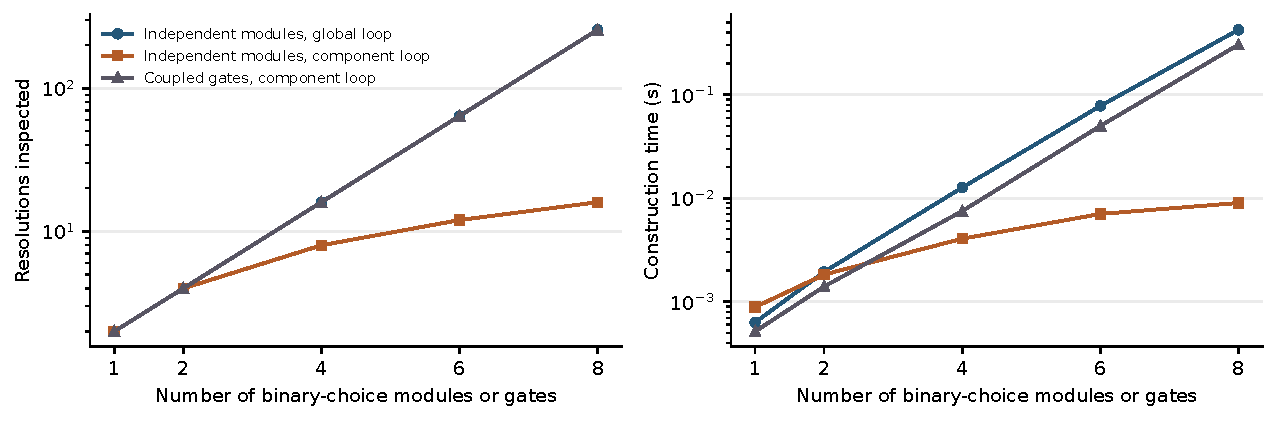
\includegraphics[width=\linewidth]{figures/scaling.pdf}
\caption{Resolutions inspected (left) and instrumented construction time (right) as the number $t$ of independent binary-choice modules, or the number $k$ of coupled gates, grows. Independent modules cost a sum of local resolution counts in the component loop and a product in the global loop; coupled gates form one component and retain the exponential output requirement. Global runs stop at parameter eight under the declared cap of 256 resolutions.}
\label{fig:scaling}
\end{figure}

Three controlled families were run with operation counters and allocation tracing: deterministic systems (disjoint two-reaction cycles, and chains of increasing depth), the independent modules of Example~\ref{ex:modules}, and the coupled gates of Proposition~\ref{prop:sharp}. Global runs were capped at $256$ resolutions and larger independent systems were run in component mode only; all $29$ calls finished within a 180-second guard. Table~\ref{tab:scaling} and Figure~\ref{fig:scaling} report the results.

The counters, not the timings, carry the argument. At $t=8$ independent modules the global loop inspects $2^8=256$ resolutions and $4{,}096$ validation prunings and generates $2{,}048$ candidate occurrences, of which $2{,}032$ are duplicates of the $16$ distinct outputs; the component loop inspects $16$ resolutions and $32$ prunings for the same $16$ outputs. At $t=64$ the component loop uses $128$ resolutions for $128$ outputs on $192$ reactions, while the global product $2^{64}$ is computed as a parameter and never enumerated. At $k=8$ coupled gates both loops use $256$ resolutions for $256$ distinct outputs, as Proposition~\ref{prop:sharp} requires. The deterministic runs show zero-excess systems of $128$ reactions handled in one resolution, and the chain family shows generation depth $128$ without supplier ambiguity. Raw records also give an incidence-count proxy and the serialized input length; neither is equated with the abstract bit length $N$.

\section{Discussion}\label{sec:discussion}

\subsection{What the theorem says}

Supplier excess is a computable, input-side parameter that controls the complete minimal family while permitting arbitrarily deep food-generation structure. Its exponential dependence is necessary on the coupled family when every output is written explicitly. The overlap theorem explains both the sharper validation account and the bounded coverage that drives the intervention guarantee. Incidence separation refines the parameter to local ambiguity and removes unnecessary combinations. Reaction restriction, counting, minimum-size and minimum-nonnegative-cost RAFs, required/forbidden queries, deletion survival and destructive cuts all reduce to scans of the catalogue. The exponential-output family and the two-cycle family show, respectively, that the catalogue can be large when the parameter is, and that the dual catalogue of minimal cuts can be large even when the parameter and the catalogue are small.

\subsection{What the theorem does not say}

The proved object is the exact family of original irreducible RAFs under the ordinary finite semantics of Section~\ref{sec:defs}. Structural minimality asserts nothing about kinetic productivity, thermodynamic realizability, concentrations, persistence, gene essentiality or fitness. Filtering the catalogue by a stronger property can miss a larger RAF that is minimal for that stronger property, as the union example of Section~\ref{sec:restriction} shows. The component criterion is sufficient, not necessary: systems sharing nonfood species across modules may be tractable for other reasons, but Theorem~\ref{thm:components} does not split them. No polynomial delay is claimed without parameter-dependent preprocessing, no extracted implementation is claimed, and no biological data study is reported. Nothing here reopens the unrestricted classification of \cite{classification2026}.

\subsection{Supplier excess and width}\label{sec:width}

Bounded-width inputs admit a general logical route. On the two-sorted incidence structure with unary predicates for species, reactions and food and binary relations for reactant, product and catalyst incidence, define for a reaction set $S$ and a species set $U$
\[
 \Closed(S,U)\ \Longleftrightarrow\ F\subseteq U\ \wedge\ \forall r\in S\,\bigl(\inp(r)\subseteq U\Rightarrow\out(r)\subseteq U\bigr).
\]
Stage induction places every generated molecule in every such $U$, and the least closure is itself closed, so $x\in\cl_Q(S)$ if and only if $x$ belongs to every $U$ with $\Closed(S,U)$. Substituting into \eqref{eq:raf} and quantifying over proper nonempty subsets for minimality gives a fixed monadic second-order formula for original irreducibility, and Courcelle's enumeration theorem \cite{courcelle1990monadic,courcelle2009linear} then yields linear-delay enumeration after preprocessing on inputs of bounded incidence treewidth. Section~\ref{sec:zerofamilies} shows that the two parameters are incomparable: the gate family has pathwidth at most $7$ and unbounded $\beta$, while the dense chain has $\beta=0$ and unbounded treewidth. The metatheorem's constants are not a practical state-size result, and an explicit width-based extension oracle with a useful state representation for original minimality remains open.

\subsection{Open problems}

\begin{enumerate}[label=\textup{(\arabic*)}]
\item An explicit dynamic-programming extension oracle for original irrRAFs on bounded-width inputs, with a proved state bound and delay.
\item Preprocessing that removes irrelevant or dependent supplier choices (Remark~\ref{rem:sufficient}) while preserving every original irrRAF.
\item Streaming or memory-bounded enumeration with guarantees stronger than the buffered $O(mnL)$ storage.
\item Exact minimum-cost destructive deletion for classes beyond $\beta=0$; Corollary~\ref{cor:greedy} is an approximation.
\item Output-sensitive enumeration of all minimal destructive cuts, beyond the incremental quasi-polynomial bound inherited from \cite{fredman1996complexity}.
\item Whether the frequency bound $f_r\le L$ and the membership bound $mL$ are simultaneously attainable, and the exact extremal constant in place of $2/3$.
\item Biological instantiations under explicit reaction, food, catalyst, reversibility and gene-action conventions, and the distribution of $\beta$ and $\bmax$ on curated metabolic networks.
\end{enumerate}
These are successor directions, not missing assumptions of the supplier theorem.

\appendix
\section{Reproduction}\label{app:repro}

All reusable proofs are in \lean{proofs/RAFStructuredEnumeration/} of \cite{repository2026}. Experiment sources, verification receipts, exact test records and the raw study data are in the workspace directory \lean{problem_workspaces/}\allowbreak\lean{RAF_tractable_irrRAF_enumeration_structural_restrictions/} of the repository: \lean{experiments/supplier_enumerator.py} (global loop), \lean{experiments/component_enumerator.py} (component loop with counters), \lean{experiments/postproof_checks.py} (regression suite, independent oracle), \lean{experiments/postproof_scaling.py} (mechanism study), \lean{results/postproof_checks.json} and \lean{results/postproof_scaling.json} (records), and the receipts \lean{results/root.verify.json}, \lean{results/overlap.verify.json}, \lean{results/restriction.verify.json}, \lean{results/supplier_resolution.verify.json}, \lean{results/earliest.verify.json} and \lean{results/deterministic.verify.json}.

From the repository root, the script \lean{reproduce_postproof.ps1} in that workspace checks the locked Python environment, reruns the regression suite and the mechanism study under a process guard, audits the preserved root receipt against the current sources, and rebuilds the original manuscript; with the switch \texttt{-Recompile} it also recompiles the overlap and restriction endpoints through the strict bridge. The original \lean{reproduce.ps1} rebuilds the root itself. A receipt is produced by
\begin{small}\begin{verbatim}
python scripts/verify_proof.py proofs/RAFStructuredEnumeration/Resolution.lean \
  --declaration RAFStructuredEnumeration.supplierEnumeration_correct \
  --timeout 300 --output root.verify.json
\end{verbatim}\end{small}
and records the toolchain, the dependency manifest hash, the source hash, the elaborated type and axioms of every exported declaration, and the compiler output under \texttt{-DwarningAsError=true}.

The source of this paper is accompanied by a script that replays every printed number from the saved records and recomputes every example of Sections~\ref{sec:resolutions}--\ref{sec:cuts} with a standard-library exhaustive reference, and by the script that regenerates Table~\ref{tab:scaling} and Figure~\ref{fig:scaling} from the saved 29-run data.

\bibliographystyle{plainnat}
\bibliography{refs}

\end{document}
